\documentclass{article}\usepackage[]{graphicx}\usepackage[]{color}
%% maxwidth is the original width if it is less than linewidth
%% otherwise use linewidth (to make sure the graphics do not exceed the margin)
\makeatletter
\def\maxwidth{ %
  \ifdim\Gin@nat@width>\linewidth
    \linewidth
  \else
    \Gin@nat@width
  \fi
}
\makeatother

\definecolor{fgcolor}{rgb}{0.345, 0.345, 0.345}
\newcommand{\hlnum}[1]{\textcolor[rgb]{0.686,0.059,0.569}{#1}}%
\newcommand{\hlstr}[1]{\textcolor[rgb]{0.192,0.494,0.8}{#1}}%
\newcommand{\hlcom}[1]{\textcolor[rgb]{0.678,0.584,0.686}{\textit{#1}}}%
\newcommand{\hlopt}[1]{\textcolor[rgb]{0,0,0}{#1}}%
\newcommand{\hlstd}[1]{\textcolor[rgb]{0.345,0.345,0.345}{#1}}%
\newcommand{\hlkwa}[1]{\textcolor[rgb]{0.161,0.373,0.58}{\textbf{#1}}}%
\newcommand{\hlkwb}[1]{\textcolor[rgb]{0.69,0.353,0.396}{#1}}%
\newcommand{\hlkwc}[1]{\textcolor[rgb]{0.333,0.667,0.333}{#1}}%
\newcommand{\hlkwd}[1]{\textcolor[rgb]{0.737,0.353,0.396}{\textbf{#1}}}%

\usepackage{framed}
\makeatletter
\newenvironment{kframe}{%
 \def\at@end@of@kframe{}%
 \ifinner\ifhmode%
  \def\at@end@of@kframe{\end{minipage}}%
  \begin{minipage}{\columnwidth}%
 \fi\fi%
 \def\FrameCommand##1{\hskip\@totalleftmargin \hskip-\fboxsep
 \colorbox{shadecolor}{##1}\hskip-\fboxsep
     % There is no \\@totalrightmargin, so:
     \hskip-\linewidth \hskip-\@totalleftmargin \hskip\columnwidth}%
 \MakeFramed {\advance\hsize-\width
   \@totalleftmargin\z@ \linewidth\hsize
   \@setminipage}}%
 {\par\unskip\endMakeFramed%
 \at@end@of@kframe}
\makeatother

\definecolor{shadecolor}{rgb}{.97, .97, .97}
\definecolor{messagecolor}{rgb}{0, 0, 0}
\definecolor{warningcolor}{rgb}{1, 0, 1}
\definecolor{errorcolor}{rgb}{1, 0, 0}
\newenvironment{knitrout}{}{} % an empty environment to be redefined in TeX

\usepackage{alltt}



\usepackage[margin=0.75in]{geometry}
\usepackage{amsmath}
\usepackage{flexisym}
\usepackage{titlesec}
\IfFileExists{upquote.sty}{\usepackage{upquote}}{}
\begin{document}


\title{Math 154 Tree-based Methods Lab}
\author{Roja, Franklin, Alejandra}
\maketitle

In addition to using the kaggle data, load the data set mtcars into R via the
command data(mtcars). Try to predict the fuel efficiency (mpg) via a regression tree, and try to predict the transmission type (automatic or manual) via a classification tree. You may want to compare the regression tree to a linear model. plot(mtcars) will give you all the pairwise scatter plots. Notice that most of the relationships with MPG are non-linear. Additionally, R has a package called randomForest. The most useful function, which implements the algorithm discussed in class, is of the same name. Compare the classification rates for a random forest to that of a simple tree.

\begin{knitrout}
\definecolor{shadecolor}{rgb}{0.969, 0.969, 0.969}\color{fgcolor}\begin{kframe}
\begin{alltt}
\hlcom{# install.packages("tree")}
\hlcom{# install.packages("randomForest")}
\hlcom{# install.packages('reprtree')}
\hlkwd{library}\hlstd{(tree)}
\hlkwd{library}\hlstd{(randomForest)}
\end{alltt}


{\ttfamily\noindent\itshape\color{messagecolor}{\#\# randomForest 4.6-12}}

{\ttfamily\noindent\itshape\color{messagecolor}{\#\# Type rfNews() to see new features/changes/bug fixes.}}\begin{alltt}
\hlkwd{library}\hlstd{(datasets)}
\hlcom{# library(reprtree)}
\hlkwd{data}\hlstd{(mtcars)}
\end{alltt}
\end{kframe}
\end{knitrout}


In order to predict the fuel efficiency we implemented a regression tree and  a linear regression model to later compare results. We divided the data into a training and test set. Since the sample size is only thirty-two, the two sets only had sixteen observations. One method we used to compare the performance of both models was residual sum of squares. We consistently found that predictions made with a linear regression model had a lower residual sum of squares than those made with a regression tree. It may be due to there only being three nodes and therefore, three averages which new observations can take on. The variables that the regression tree selected were the number of cylinders and the weight of the car to create partitions. 


\begin{knitrout}
\definecolor{shadecolor}{rgb}{0.969, 0.969, 0.969}\color{fgcolor}\begin{kframe}
\begin{alltt}
\hlcom{# Regression Tree}
\hlstd{test.index} \hlkwb{=} \hlkwd{sample}\hlstd{(}\hlkwd{c}\hlstd{(}\hlnum{1}\hlopt{:}\hlkwd{nrow}\hlstd{(mtcars)),}\hlkwd{nrow}\hlstd{(mtcars)}\hlopt{/}\hlnum{2} \hlstd{)}
\hlstd{training.index}\hlkwb{=} \hlkwd{c}\hlstd{(}\hlnum{1}\hlopt{:}\hlkwd{nrow}\hlstd{(mtcars))[}\hlopt{-}\hlstd{test.index]}
\hlstd{test.data} \hlkwb{=} \hlstd{mtcars[test.index,]}
\hlstd{training.data} \hlkwb{=} \hlstd{mtcars[training.index,]}
\hlstd{cars.regression} \hlkwb{<-} \hlkwd{tree}\hlstd{(mpg} \hlopt{~} \hlstd{cyl}\hlopt{+}\hlstd{disp}\hlopt{+}\hlstd{hp}\hlopt{+}\hlstd{drat}\hlopt{+}\hlstd{wt}\hlopt{+}\hlstd{qsec}\hlopt{+}\hlstd{vs}\hlopt{+}\hlstd{am}\hlopt{+}\hlstd{gear}\hlopt{+}\hlstd{carb,} \hlkwc{data}\hlstd{=training.data)}
\hlkwd{plot}\hlstd{(cars.regression )}
\hlkwd{text}\hlstd{(cars.regression ,} \hlkwc{cex}\hlstd{=}\hlnum{.75}\hlstd{)}
\end{alltt}
\end{kframe}
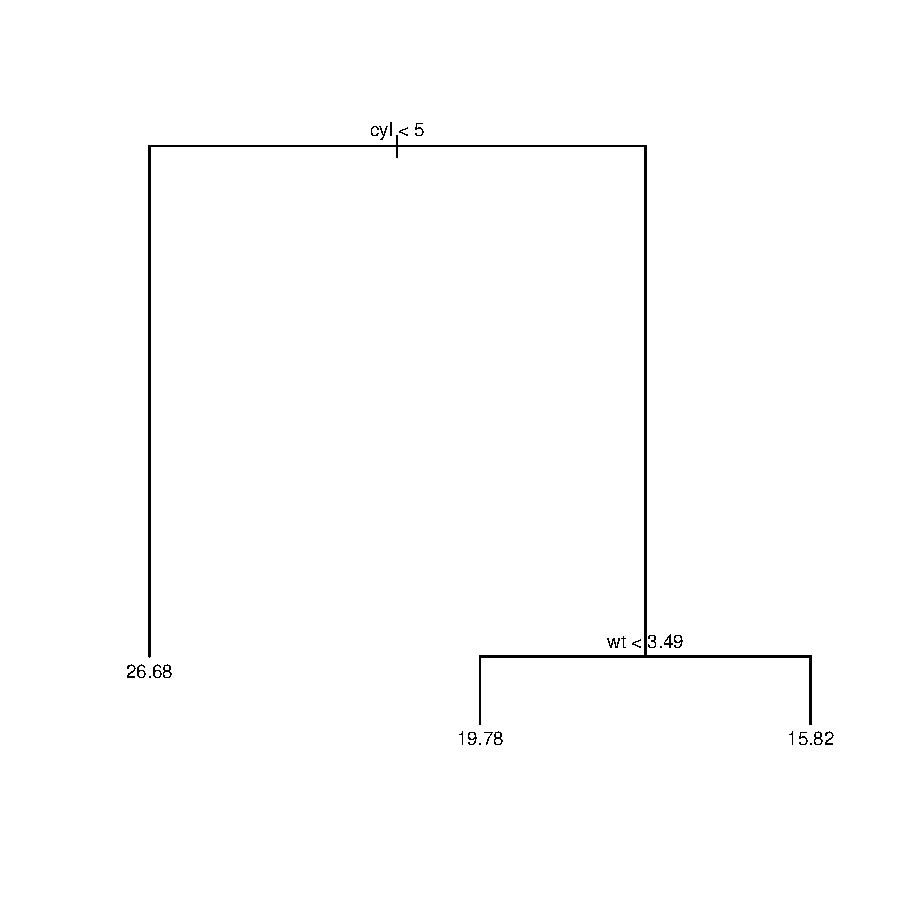
\includegraphics[width=\maxwidth]{figure/unnamed-chunk-2-1} 
\begin{kframe}\begin{alltt}
\hlstd{my.prediction} \hlkwb{<-} \hlkwd{predict}\hlstd{(cars.regression, test.data)}
\hlcom{# find RSS }
\hlstd{residuals} \hlkwb{=} \hlstd{(test.data}\hlopt{$}\hlstd{mpg} \hlopt{-} \hlstd{my.prediction)}\hlopt{^}\hlnum{2}
\hlkwd{sum}\hlstd{(residuals}\hlopt{^}\hlnum{2}\hlstd{)}
\end{alltt}
\begin{verbatim}
## [1] 7015.598
\end{verbatim}
\begin{alltt}
\hlcom{# plot residuals }
\hlkwd{par}\hlstd{(}\hlkwc{mfrow}\hlstd{=}\hlkwd{c}\hlstd{(}\hlnum{2}\hlstd{,}\hlnum{2}\hlstd{))}
\hlkwd{plot}\hlstd{(residuals,} \hlkwc{main}\hlstd{=} \hlstr{'Residuals from Regression Tree'}\hlstd{)}
\hlcom{# plot of actual and predictions}
\hlkwd{plot}\hlstd{(test.data}\hlopt{$}\hlstd{mpg,} \hlkwc{ylim} \hlstd{=} \hlkwd{c}\hlstd{(}\hlnum{0}\hlstd{,}\hlnum{40}\hlstd{),} \hlkwc{main} \hlstd{=} \hlstr{' Predictions and Actual'}\hlstd{)}
\hlkwd{points}\hlstd{(my.prediction,} \hlkwc{col} \hlstd{=} \hlstr{'red'}\hlstd{)}
\hlkwd{legend}\hlstd{(}\hlnum{2}\hlstd{,} \hlnum{10}\hlstd{,} \hlkwc{legend}\hlstd{=}\hlkwd{c}\hlstd{(}\hlstr{"Actual"}\hlstd{,} \hlstr{"Predictions"}\hlstd{),}
       \hlkwc{col}\hlstd{=}\hlkwd{c}\hlstd{(}\hlstr{"black"}\hlstd{,} \hlstr{"red"}\hlstd{),}\hlkwc{pch} \hlstd{=} \hlnum{1}\hlstd{)}
\hlcom{#####}
\hlcom{# Comparing to a Linear model }
\hlstd{cars.lm} \hlkwb{<-} \hlkwd{lm} \hlstd{( mpg} \hlopt{~} \hlstd{cyl}\hlopt{+}\hlstd{disp}\hlopt{+}\hlstd{hp}\hlopt{+}\hlstd{drat}\hlopt{+}\hlstd{wt}\hlopt{+}\hlstd{qsec}\hlopt{+}\hlstd{vs}\hlopt{+}\hlstd{am}\hlopt{+}\hlstd{gear}\hlopt{+}\hlstd{carb,} \hlkwc{data}\hlstd{= training.data)}
\hlstd{prediction.lm} \hlkwb{<-} \hlkwd{predict}\hlstd{(cars.lm, test.data)}
\hlcom{# find RSS }
\hlstd{residuals.lm} \hlkwb{=} \hlstd{(test.data}\hlopt{$}\hlstd{mpg} \hlopt{-} \hlstd{prediction.lm)}\hlopt{^}\hlnum{2}
\hlkwd{sum}\hlstd{(residuals.lm}\hlopt{^}\hlnum{2}\hlstd{)}
\end{alltt}
\begin{verbatim}
## [1] 2472197
\end{verbatim}
\begin{alltt}
\hlcom{# plot residuals }
\hlkwd{plot}\hlstd{(residuals.lm,} \hlkwc{main} \hlstd{=} \hlstr{"Residuals from Linear Model"}\hlstd{)}
\hlcom{# plot of actual and predictions}
\hlkwd{plot}\hlstd{(test.data}\hlopt{$}\hlstd{mpg,} \hlkwc{main}\hlstd{=} \hlstr{" Actual vs. Prediction from Linear Model"}\hlstd{,} \hlkwc{ylim} \hlstd{=} \hlkwd{c}\hlstd{(}\hlnum{0}\hlstd{,}\hlnum{40}\hlstd{))}
\hlkwd{points}\hlstd{(prediction.lm,} \hlkwc{col} \hlstd{=} \hlstr{'red'}\hlstd{)}
\hlkwd{legend}\hlstd{(}\hlnum{2}\hlstd{,} \hlnum{10}\hlstd{,} \hlkwc{legend}\hlstd{=}\hlkwd{c}\hlstd{(}\hlstr{"Actual"}\hlstd{,} \hlstr{"Predictions"}\hlstd{),}
       \hlkwc{col}\hlstd{=}\hlkwd{c}\hlstd{(}\hlstr{"black"}\hlstd{,} \hlstr{"red"}\hlstd{),}\hlkwc{pch} \hlstd{=} \hlnum{1}\hlstd{)}
\end{alltt}
\end{kframe}
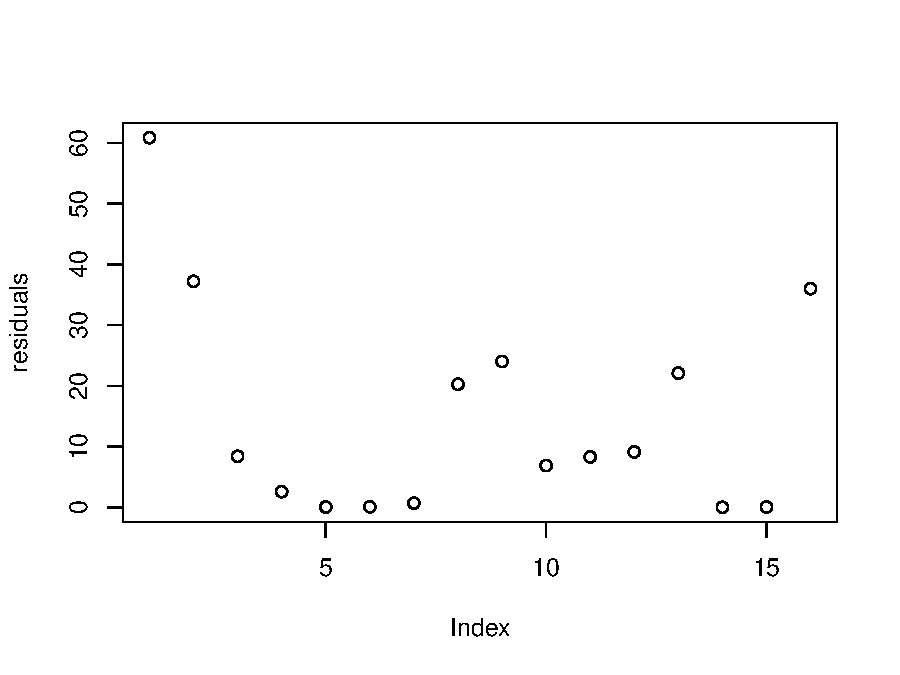
\includegraphics[width=\maxwidth]{figure/unnamed-chunk-2-2} 

\end{knitrout}


We used Classification and Random Forests to predict the transmission type of a car. The classification tree had two terminal nodes and used \textit{weight} as a point of partition. Since the response variable was binary we calculated the proportion of times each method predicted  accurately. The accuracy of the predictions from both methods were about the same. To compare the success rates of both we ran multiple simulations and recorded the proportion of successes. After running the simulation below several times we observed that random forests provided consistently had less incorrect predictions. 

\begin{knitrout}
\definecolor{shadecolor}{rgb}{0.969, 0.969, 0.969}\color{fgcolor}\begin{kframe}
\begin{alltt}
\hlcom{# Classification Tree}
\hlcom{# Use a classification tree to predict transmission type of car}
\hlcom{# Transmission (0 = automatic, 1 = manual)}

\hlstd{incorrect.predict.Forest} \hlkwb{=} \hlkwd{c}\hlstd{()}
\hlstd{incorrect.predict.class} \hlkwb{=} \hlkwd{c}\hlstd{()}
\hlkwa{for} \hlstd{(i} \hlkwa{in} \hlkwd{c}\hlstd{(}\hlnum{1}\hlopt{:}\hlnum{40}\hlstd{))\{}
\hlstd{test.index} \hlkwb{=} \hlkwd{sample}\hlstd{(}\hlkwd{c}\hlstd{(}\hlnum{1}\hlopt{:}\hlkwd{nrow}\hlstd{(mtcars)),}\hlkwd{nrow}\hlstd{(mtcars)}\hlopt{/}\hlnum{2} \hlstd{)}
\hlstd{training.index}\hlkwb{=} \hlkwd{c}\hlstd{(}\hlnum{1}\hlopt{:}\hlkwd{nrow}\hlstd{(mtcars))[}\hlopt{-}\hlstd{test.index]}

\hlstd{test.data} \hlkwb{=} \hlstd{mtcars[test.index,]}
\hlstd{training.data} \hlkwb{=} \hlstd{mtcars[training.index,]}

\hlstd{cars.class}\hlkwb{<-}\hlkwd{tree}\hlstd{(am} \hlopt{~} \hlstd{mpg}\hlopt{+}\hlstd{cyl}\hlopt{+}\hlstd{disp}\hlopt{+}\hlstd{hp}\hlopt{+}\hlstd{drat}\hlopt{+}\hlstd{wt}\hlopt{+}\hlstd{qsec}\hlopt{+}\hlstd{vs}\hlopt{+}\hlstd{gear}\hlopt{+}\hlstd{carb,} \hlkwc{data}\hlstd{=training.data)}
\hlkwd{summary}\hlstd{(cars.class)}

\hlstd{my.prediction.class} \hlkwb{<-} \hlkwd{predict}\hlstd{(cars.class, test.data)}
\hlstd{my.prediction.class[(my.prediction.class} \hlopt{<} \hlnum{0.5}\hlstd{)]} \hlkwb{=} \hlnum{0}
\hlstd{my.prediction.class[(my.prediction.class} \hlopt{>} \hlnum{0.5}\hlstd{)]} \hlkwb{=} \hlnum{1}
\hlcom{# how many incorrect predictions }
\hlstd{incorrect.predict.class[i]} \hlkwb{=} \hlkwd{sum}\hlstd{(}\hlkwd{abs}\hlstd{(my.prediction.class} \hlopt{-} \hlstd{test.data}\hlopt{$}\hlstd{am)} \hlopt{>} \hlnum{.5}\hlstd{)}

\hlcom{####}
\hlcom{# Using a Random Forest}
\hlstd{cars.Forest} \hlkwb{<-} \hlkwd{randomForest}\hlstd{(}\hlkwd{as.factor}\hlstd{(am)} \hlopt{~} \hlstd{mpg}\hlopt{+}\hlstd{cyl}\hlopt{+}\hlstd{disp}\hlopt{+}\hlstd{hp}\hlopt{+}\hlstd{drat}\hlopt{+}\hlstd{wt}\hlopt{+}\hlstd{qsec}\hlopt{+}\hlstd{vs}\hlopt{+}\hlstd{gear}\hlopt{+}\hlstd{carb,} \hlkwc{data}\hlstd{=training.data ,} \hlkwc{importance}\hlstd{=}\hlnum{TRUE}\hlstd{,}
                            \hlkwc{ntree}\hlstd{=}\hlnum{128}\hlstd{)}
\hlstd{prediction.Forest}\hlkwb{<-} \hlkwd{predict}\hlstd{(cars.Forest, test.data)}
\hlcom{# how many incorrect predictions }
\hlstd{incorrect.predict.Forest[i]} \hlkwb{=} \hlkwd{sum}\hlstd{(}\hlkwd{abs}\hlstd{((}\hlkwd{as.numeric}\hlstd{(prediction.Forest)} \hlopt{-} \hlnum{1}\hlstd{)} \hlopt{-} \hlstd{test.data}\hlopt{$}\hlstd{am)} \hlopt{>} \hlnum{.5}\hlstd{)}
\hlstd{\}}

\hlkwd{plot}\hlstd{(cars.class, ,} \hlkwc{main}\hlstd{=} \hlstr{'Classification Results'}\hlstd{)}
\hlkwd{text}\hlstd{(cars.class)}
\end{alltt}
\end{kframe}
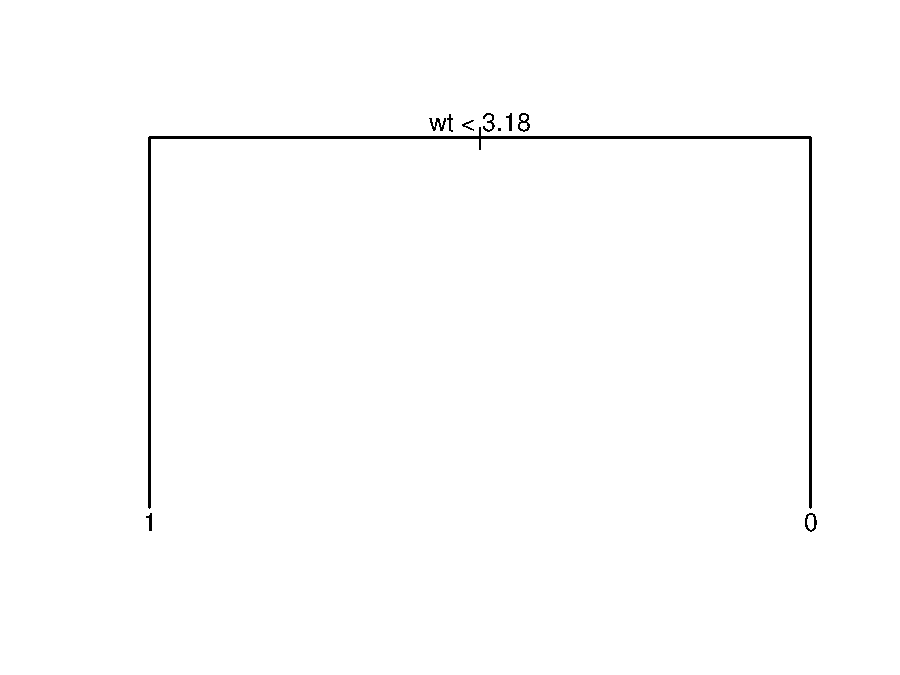
\includegraphics[width=\maxwidth]{figure/unnamed-chunk-3-1} 
\begin{kframe}\begin{alltt}
\hlkwd{plot}\hlstd{(test.data}\hlopt{$}\hlstd{am,} \hlkwc{ylim} \hlstd{=} \hlkwd{c}\hlstd{(}\hlnum{0}\hlstd{,}\hlnum{1}\hlstd{),} \hlkwc{main}\hlstd{=} \hlstr{'Results from Classification Tree'}\hlstd{)}
\hlkwd{points}\hlstd{(my.prediction.class,}\hlkwc{col} \hlstd{=} \hlstr{'purple'}\hlstd{,} \hlkwc{pch} \hlstd{=} \hlstr{"."}\hlstd{)}
\hlkwd{legend}\hlstd{(}\hlnum{1}\hlstd{,} \hlnum{0.4}\hlstd{,} \hlkwc{legend}\hlstd{=}\hlkwd{c}\hlstd{(}\hlstr{"Actual"}\hlstd{,} \hlstr{"Predictions"}\hlstd{),}
       \hlkwc{col}\hlstd{=}\hlkwd{c}\hlstd{(}\hlstr{"black"}\hlstd{,} \hlstr{"purple"}\hlstd{),}\hlkwc{pch} \hlstd{=} \hlnum{1}\hlstd{)}
\end{alltt}
\end{kframe}
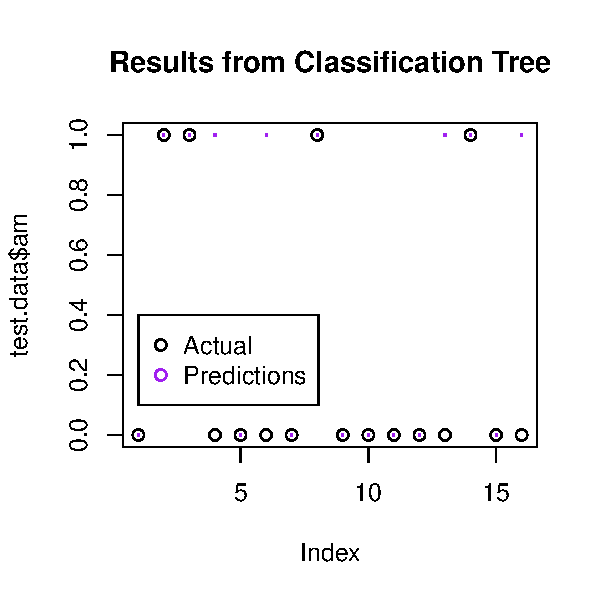
\includegraphics[width=\maxwidth]{figure/unnamed-chunk-3-2} 
\begin{kframe}\begin{alltt}
\hlkwd{plot}\hlstd{(test.data}\hlopt{$}\hlstd{am,} \hlkwc{main}\hlstd{=} \hlstr{'Results from Random Forest'}\hlstd{)}
\hlkwd{points}\hlstd{(}\hlkwd{as.numeric}\hlstd{(prediction.Forest)}\hlopt{-}\hlnum{1}\hlstd{,}\hlkwc{col} \hlstd{=} \hlstr{'purple'}\hlstd{,} \hlkwc{pch} \hlstd{=} \hlstr{"."}\hlstd{)}
\hlkwd{legend}\hlstd{(}\hlnum{1}\hlstd{,} \hlnum{0.4}\hlstd{,} \hlkwc{legend}\hlstd{=}\hlkwd{c}\hlstd{(}\hlstr{"Actual"}\hlstd{,} \hlstr{"Predictions"}\hlstd{),}
       \hlkwc{col}\hlstd{=}\hlkwd{c}\hlstd{(}\hlstr{"black"}\hlstd{,} \hlstr{"purple"}\hlstd{),}\hlkwc{pch} \hlstd{=} \hlnum{1}\hlstd{)}
\end{alltt}
\end{kframe}
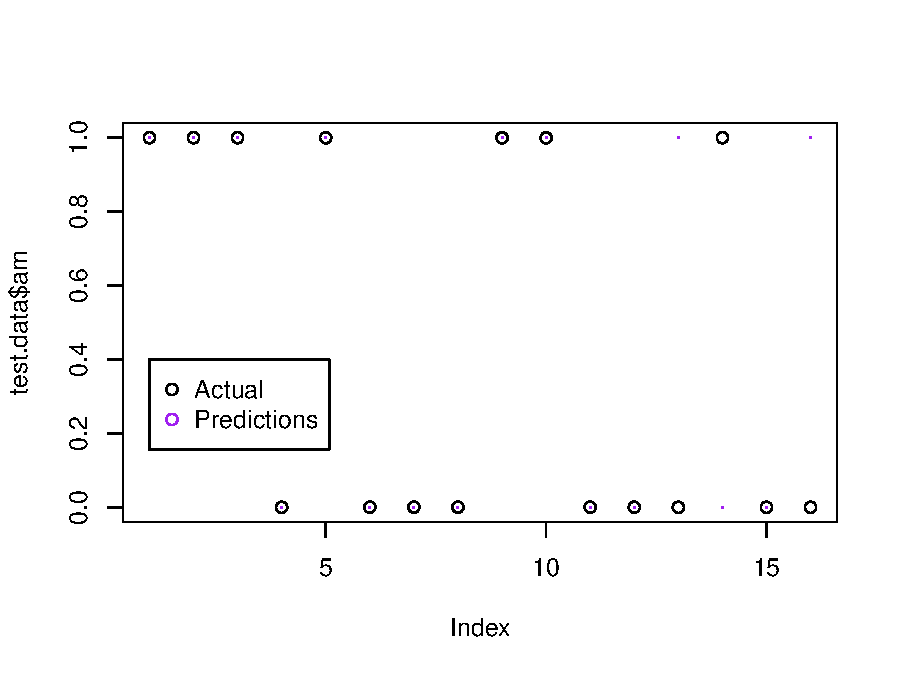
\includegraphics[width=\maxwidth]{figure/unnamed-chunk-3-3} 
\begin{kframe}\begin{alltt}
\hlstd{incorrect.predict.Forest}
\end{alltt}
\begin{verbatim}
##  [1] 0 5 5 4 2 2 3 3 4 4 2 3 5 2 2 1 5 5 1 1 4 4 4 1 3 1 4 2 6 1 4 5 5 3 4
## [36] 2 3 3 1 3
\end{verbatim}
\begin{alltt}
\hlstd{incorrect.predict.class}
\end{alltt}
\begin{verbatim}
##  [1] 1 6 4 2 2 3 2 4 4 4 4 5 5 3 3 3 6 3 2 2 5 0 5 1 4 2 2 2 4 2 6 2 2 3 4
## [36] 3 3 3 2 4
\end{verbatim}
\begin{alltt}
\hlkwd{mean}\hlstd{(incorrect.predict.Forest)}
\end{alltt}
\begin{verbatim}
## [1] 3.05
\end{verbatim}
\begin{alltt}
\hlkwd{mean}\hlstd{(incorrect.predict.class)}
\end{alltt}
\begin{verbatim}
## [1] 3.175
\end{verbatim}
\end{kframe}
\end{knitrout}





\end{document}
